%%%%%%%%%%%%%%%%%%%%%%%%%%%%%%%%%%%%%%%%%%%%%%%%%%%%%%%%%%%%%%%%%%%%%%%%%%%
% Copyright (c) 2010 committers of YAKINDU and others.
% All rights reserved. This program and the accompanying materials
% are made available under the terms of the Eclipse Public License v1.0
% which accompanies this distribution, and is available at
% http://www.eclipse.org/legal/epl-v10.html
%
% Contributors:
%     committers of YAKINDU - initial API and implementation
%%%%%%%%%%%%%%%%%%%%%%%%%%%%%%%%%%%%%%%%%%%%%%%%%%%%%%%%%%%%%%%%%%%%%%%%%%%
\section{Eclipse Installation}

The YAKINDU Plugin installation follows the usual eclipse installation process.

However, before you start, be sure to have the Eclipse environment (3.5/Galileo)
installed. You can download eclipse distributions from the Eclipse download site.

\url{http://www.eclipse.org/downloads/}

Please be aware that there are many different distributions supporting different
features. When installing the YAKINDU features the required features will be
installed automatically if they are not already installed. You can also download
the itemis oAW distribution that already contains several required plugins.

%\url{http://oaw.itemis.com/openarchitectureware/language=en/2837/downloads}
\url{http://oaw.itemis.com/downloads/}

The YAKINDU statechart tools require several Eclipse plugins:

\begin{itemize}
\item EMF
\item GEF
\item GMF
\item Xtend
\item Xpand
\item Xtext
\item MWE
\item and some others\dots
\end{itemize}

Additionally you may want to install additional features like the CDT (C/C++
Development Tools) or the JDT (Java Development Tools). You can install them with
the same mechanism as described in the next section.

\section{Installing the YAKINDU-Plugins}

To install the YAKINDU plugins, open the \textbf{Software Updates and Add-Ons}
dialog which can be found at Help$\rightarrow$ \textbf{Install New Software...} (like
\ref{fig:updatesMenu}). \begin{figure}[ht] \center

\includegraphics[width=0.3\textwidth]{Pictures/helpMenu}\\
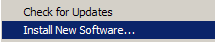
\includegraphics[width=0.3\textwidth]{Pictures/softwareUpdates}
\caption{\label{fig:updatesMenu}Menu to select software updates} 
\end{figure}
In the window press the \textbf{Add ...} button and enter the update site URL
% http://vm0a:8080/job/YAKINDU\%20Update-Site/ws/update/
\url{http://updates.yakindu.com/galileo/release/}
into the \textit{Location} area (see Figure \ref{fig:updateSite}). After
accepting the new URL the update site will be queried.

\begin{figure}[ht]
\center
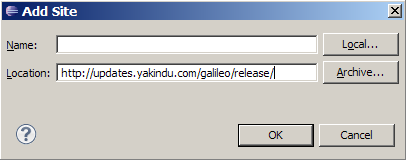
\includegraphics[width=0.7\textwidth]{./Pictures/updateSite}
\caption{\label{fig:updateSite}Update site for YAKINDU} 
\end{figure}

If everything is correct, you will find a new entry \textit{YAKINDU Update Site}
in the list in the \textit{Available Software} tab. Before continue it is
neccessary to acitvate update sites for MWE, Xpand and Xtext. This is
done by clicking on \textbf{Manage Sites\dots} and selecting the Galileo update site.
\begin{figure}[ht]
\center 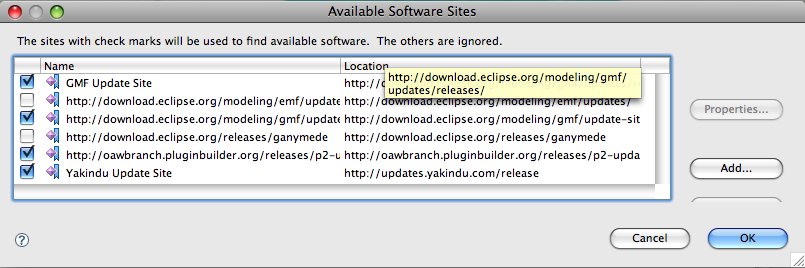
\includegraphics[width=0.5\textwidth]{./Pictures/manageSites}
\caption{\label{fig:manageSites}Select update site for dependency resolving} 
\end{figure}

For quick start check the Feature \textit{YAKINDU Feature}, \textit{MWE SDK}, 
\textit{Xpand SDK} and \textit{Xtext SDK} below the tree of
\textit{YAKINDU Update Site} and \textit{Galileo Update Site}. After select the 
Features press the \textbf{Install} button. For  the
first installation many dependencies are downloaded and you have to wait some
minutes.

\begin{figure}[ht]
\center
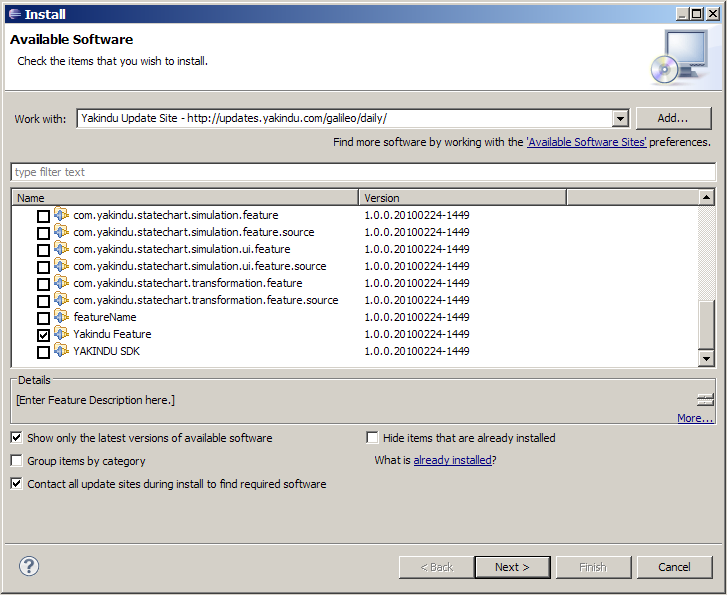
\includegraphics[width=0.45\textwidth]{./Pictures/updateSelected}
\caption{\label{fig:Update}Software Updates and Add-Ons Install Dialog} 
\end{figure}

In the next steps you have to confirm the selected Features (see Figure
\ref{fig:confirmFeatures}) and accept the License after reading it. Confirm the Security
Warning by clicking the "Ok" button. The next
steps are automatic and are finished by an information box from eclipse, asking
you to restart. Answer with \textit{Yes}, because YAKINDU becomes active after
restart.

\begin{figure}[ht] \center
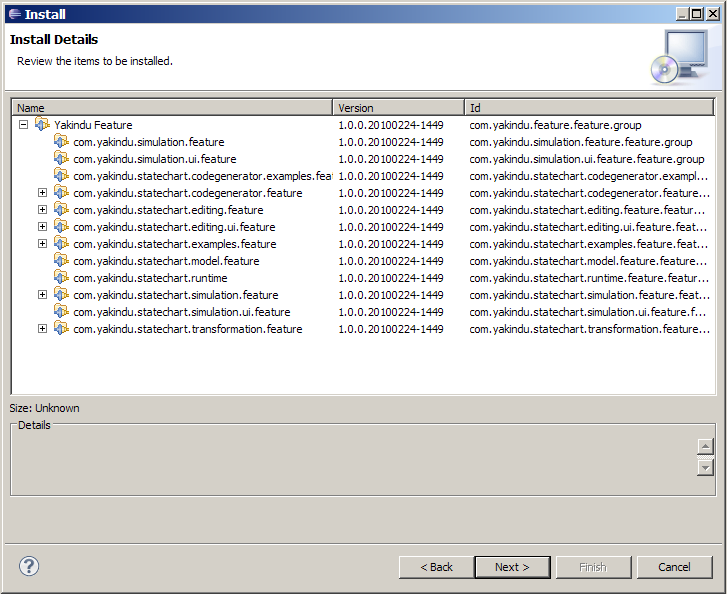
\includegraphics[width=0.45\textwidth]{./Pictures/featureConfirm}
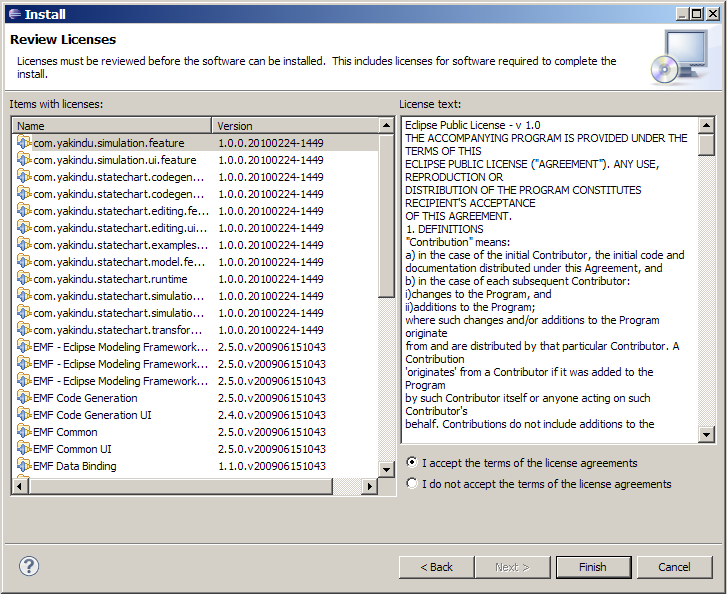
\includegraphics[width=0.45\textwidth]{./Pictures/licences}
\caption{\label{fig:confirmFeatures}Confirm selected features and the license} 
\end{figure}

After a few seconds, your installation is ready to run the quick start example
presented in the next section. Before we continue it is a good idea to change the
perspective to YAKINDU. With this perspective all main tools from the
YAKINDU-Toolchain are directly accessible. Although it's also possible to add
some of this views to your favourite perspective and edit statecharts in parallel
to your all day work.

It is highly recommended that you update your plugins after installation via 
\textit{Help}$\rightarrow$ \textit{Check for Updates}. So you get the actual
version of the YAKINDU-Statechart Tools.

\newpage
\section{Installing from Zip}

The YAKINDU-Web Site also provides a zip file with all plugins for download. The
dependencies to GMF must be satisfied manually. The update sites for eclipse 
are the following and the required features are mostly the sdks of the plugins 
mentioned before:

\begin{itemize}
\item EMF Update Site: \url{http://download.eclipse.org/modeling/emf/updates/}
\item GMF Update Site: \url{http://download.eclipse.org/modeling/gmf/updates/releases/}
\item Galileo Update Site: http://download.eclipse.org/releases/galileo
\item Xtext \url{http://xtext.itemis.com/downloads/}
\item and some others\dots
\end{itemize}

